\documentclass[12pt]{extarticle}
\usepackage[utf8]{inputenc}
\usepackage{amsmath}
\usepackage{hyperref}
\usepackage[shortlabels]{enumitem}
\usepackage{tikz}
\usepackage{textcomp}

\addtolength{\textwidth}{1.0in}
\addtolength{\textheight}{0.75in}
\addtolength{\evensidemargin}{-0.75in}
\addtolength{\oddsidemargin}{-0.75in}
\addtolength{\topmargin}{-1.0in}

\title{Analytic Geometry - Answers}
\author{Eric Xiao}
\date{May 2, 2020}

\begin{document}

\maketitle

%\section{Recall}
%\begin{itemize}
    %\item {Slope between ($x_1$, $y_1$) and ($x_2$, $y_2$) = $\frac{y_2 - y_1}{x_2 - x_1}$}
    %\item {Parallel lines have equal slopes, and product of two perpendicular slopes is -1 (negative reciprocals)}
    %\item {Distance between ($x_1$, $y_1$) and ($x_2$, $y_2$) = $\sqrt{(x_2 - x_1)^2 + (y_2 - y_1)^2}$}
    %\item {Distance between ($x_1$, $y_1$) and line $ax + by + c = 0$ = $\frac{|ax_1 + by_1 + c|}{\sqrt{a^2 + b^2}}$}
    %\item {Midpoint between ($x_1$, $y_1$) and ($x_2$, $y_2$) = ($\frac{x_1 + x_2}{2}$, $\frac{y_1 + y_2}{2}$)}
    %\item {Equation of a circle: $(x-a)^2 + (y-b)^2 = r^2$
    %\begin{itemize}
        %\item {($a$, $b$) is the centre's coordinates}
        %\item {$r$ is the circle's radius}
    %\end{itemize}}
    %\item {Triangle area with vertices ($x_1$, $y_1$), ($x_2$, $y_2$), and ($x_3$, $y_3$) = $\frac{1}{2}$$|x_1y_2 + x_2y_3 + x_3y_1 - x_2y_1 - x_3y_2 - x_1y_3|$}
%\end{itemize}

\section{Problems}
\begin{enumerate}
    \itemsep 2.0em
    \item {The midpoint between $P$($x$, $y$) and (10, 15) is (6, 4). Find the numerical coordinates of point $P$. \\Answer: \fbox{(2, -7)}}
    \item {Find the equation of a line in standard form that is perpendicular to $4x - 3y = 0$ and is a distance of 8 units away from the point (4, 6). \\Answer: \fbox{$3x + 4y + 4 = 0$} or \fbox{$3x + 4y - 76 = 0$}}
    \item {Find the equation of the circle with center (3,7) and area $17\pi$ units. \\Answer: \fbox{$(x-3)^2 + (y-7)^2 = 17$}}
    \item {A vertical line divides the triangle with vertices $O$(0, 0), $C$(9, 0) and $D$(8, 4) into two regions of equal area. Find the equation of the line. \\Answer: \fbox{$x = 6$ or $x - 6 = 0$}}
    \item {Given the circles $x^2 + y^2 = 4$ and $x^2 + y^2 - 6x + 2 = 0$, find the length of their common chord. \\Answer: \fbox{2$\sqrt{3}$}}
    \item {\textbf{Question from the 2018 CSMC:} Alexandra draws a letter A which stands on the $x$-axis.
    \begin{enumerate}
        \itemsep 2.0em
        \item {The left side of the letter A lies along the line with equation $y = 3x + 6$. What is the $x$-intercept of the line with equation $y = 3x + 6?$\\
        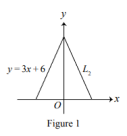
\includegraphics{CSMC2018_B1a.png} Answer: \fbox{-2}}
        \item {The right side of the letter A lies along the line $L_2$ and the letter is symmetric about the $y$-axis. What is the equation of line $L_2$? \\Answer: \fbox{$y = -3x + 6$}}
        \item {Determine the area of the triangle formed by the $x$-axis and the left and right sides of the letter A. \\Answer: \fbox{12}}
        \item {Alexandra completes the letter A by adding to Figure 1. She draws the horizontal part of the letter A along the line $y = c$, as in Figure 2. The area of the shaded region inside the letter A and above the line with equation $y = c$ is $\frac{4}{9}$ of the total area of the region above the $x$-axis and between the left and right sides. Determine the value of $c$.\\
        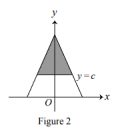
\includegraphics{CSMC2018_B1d.png} Answer: \fbox{2}}
    \end{enumerate}}
\end{enumerate}

\end{document}
